% !TEX root = DesignDocument.tex


\section{Sprint Report \#1}
Sprint Report \#1


\subsection{Team Members:}
Dicheng Wu
\\Marcus Berger\\
\textbf{Sponsor:}
\\Jeff McGough
\\

\subsection{Customer description}

\subsubsection{Description of sponsoring customer}
The sponsoring customer for this project is Dr. Jeff McGough a computer science professor at the South Dakota School of Mines and Technology and the vice president of the Academy of Dance Arts in Rapid City, South Dakota. Well not the sponsor of the project Dr. McGough's wife is also a key part of the customer base as the owner of the Academy. She and other dance school owner are the target group for this project. 

\subsubsection{Statement of customer's problem or goal for this project}
The customer wants a software that can run the day to day operations of a dance studio and also handle record keeping, billing, payroll, and other business operations
 
\subsubsection{Customer's Needs}
The customer needs us to develop a software solution which can run the dance studio in an effective manner. The product also needs to handle changing classes from year to year without needing to be updated. This means that the software needs to sync with multiple users, and handle new information such as class rosters, prices, clothing requirements for classes, changes in the employment roster, and many other changes that can occur in the running of a dance school.\\
This project as a whole needs to be an improvement on the current system in use by the customer and provide an easy and efficient way to run the clients business. 



\subsection{Overview of the project:}
The project consists of three major parts, Gui, database and back end code. For the Gui part, we are going to integrate everything into a small number of windows to eliminate the need for large numbers of window like the current product in use at the academy. and, thus, users can manipulate it very straightforwardly. For database part, we are going to build a database which stores students, employees, classes, billing, and other information needed for the academy to function as a business. For the code back end, we are going to develop it on using Python and PyQt with a primary focus on Mac but with cross platform compatibles. 

\subsection{Project Environment:}

\subsubsection{Project boundaries}
The boundaries of this project would be the Academy of Dance Arts in Rapid City. The product could be used by other dance schools in the future but they are out of the scope of this projects development 

\subsubsection{Project context}
The context of this project is only to develop a better software solution to the current software in use at the Academy of Dance Arts in Rapid City, South Dakota, so they can run their school in a more efficient manner. While the project is open source it is not the intention of this team to develop an all purpose solution for all the dance schools around the country. This project is tailored to the needs of the Academy of Dance Arts.


\subsection{Project deliverables of Sprint 1:}

\begin{enumerate}
\item The research into program languages, database and Gui frameworks and architectures for the DanceSoft project.
\item Final decision on frameworks and architectures for the DanceSoft project.
\item User Stories and Product Backlogs for the project.
\item Creating a very simple Qt window.
\end{enumerate}

\subsection{User Stories}

After the requirement for the project were laid out the team created the user stories based on those requirement. The user stories the team came up with are as fallows:

\begin{enumerate}
  \item As a user i want to adjust students payment models
  \item As the owner I would like to see automatic database backups.
  \item As a student I would like to be able to register online (with special app). Classes must be approved before added.
  \item As a student I would like to be able to search clothing requirements.
  \item As a student I would like to know my billing.
  \item As the owner I would like to indicate clothing requirements per class.
  \item As a studio person, I would like to be able to add students to classes.
  \item  As a student, teacher etc, I would like to be able to look up a students class list.
  \item As the teacher I would like to get a class role for each class.
  \item Given a class list, I would like to get an invoice of the tuition due.
  \item Studio would like to track payments and estimate remainder due.  I would like to generate an invoice for this amount.
  \item As a student I would like to be able to register online (with special app).   Classes must be approved before added.
  \item As a student I would like to know my billing.
  \item As the owner I would like to track teacher hours and compute payroll.
  \item As the owner I would like to indicate clothing requirements per class.
  \item As a student I would like to be able to search clothing requirements.
  \item As the owner I would like to see automatic database backups.
\end{enumerate}

\subsection{Product Backlog:}

From the above user stories the team produced the fallowing product backlog. The parts are not in the order of execution. More thing will be add or removed to this in the future as the software develops.

\begin{enumerate}
\item Create the database tables
\item Create database backup system
\item Create online register page and approval system
\item create clothing requirement update function, and add clothing function for teachers and admin
\item create clothing viewer function for students
\item create dynamic billing algorithms (expand on later sprint)
\item create page for tuition calculation and viewing by students
\item Add and subtract students from a class
\item Create dynamic Queries to produce class attendance list
\item Hour tracker for teachers and payroll calculation algorithm (expanded later)
\item Using dynamic DNS service to set up Linux Box
\item Encrypt data that store in the database
\item retrieve data from database to produce a invoice for payroll
\item queries in database to retrieve student information
\item Create ability for employee to look up and modify student registration info
\item Query database to produce class role sheet
\item Query database to produce employee information
\item create permission assignment system
\item handle billing info (expand later)
\item Create dynamic algorithm for payment model creation and calculation. 
\item Algorithm for payment tracking and remainder calculation, and query database to produce invoice.
\item Query and insert information needed to create and new class and produce a results page.
\item Create update query to assign teachers to a class
\end{enumerate}

\begin{figure}
\caption{DanceSoft Trello Board}
\centering
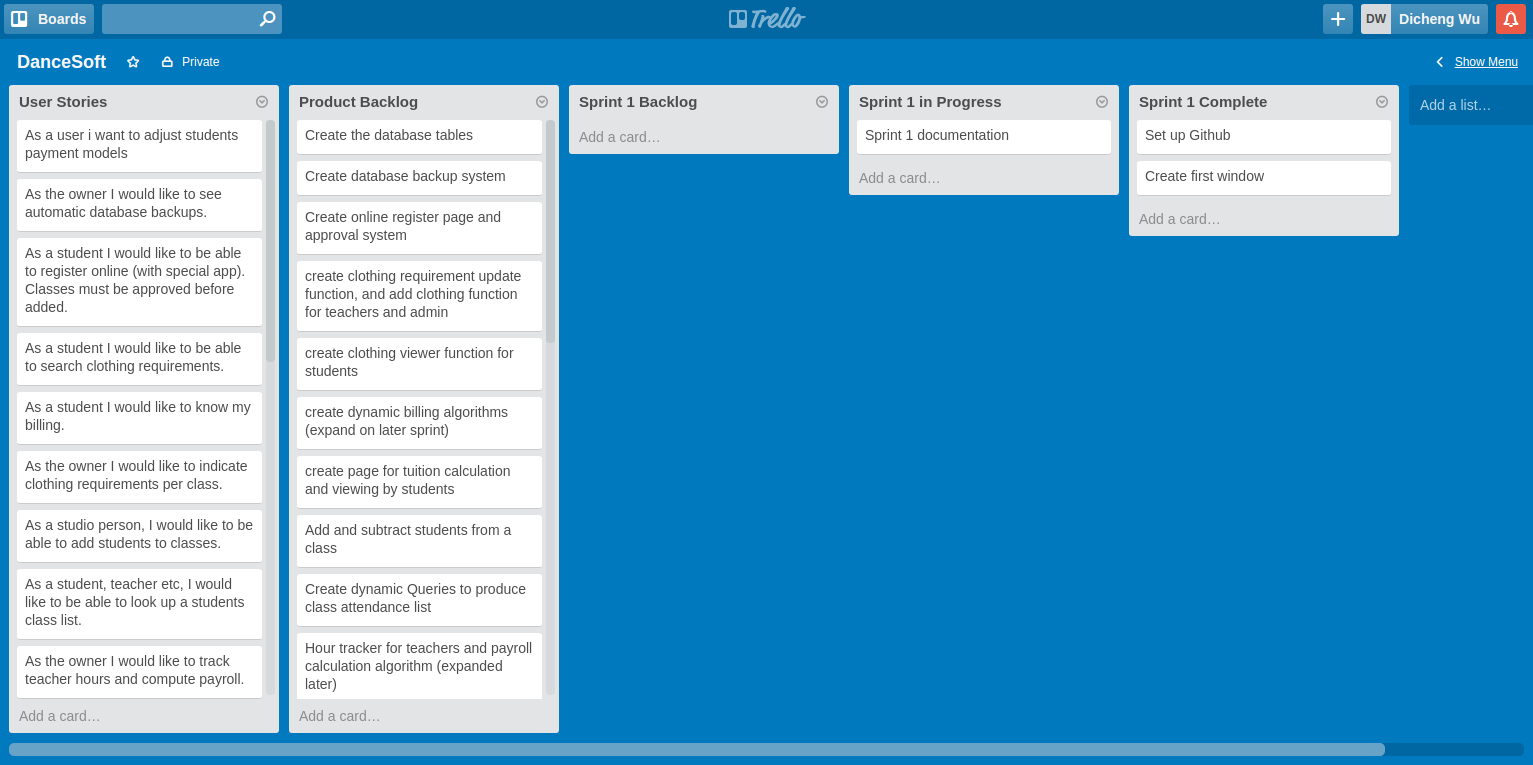
\includegraphics[width=0.5\textwidth]{d1}
\end{figure}



\subsubsection{Sprint 1 Backlog:}

\begin{enumerate}
\item Set up Github
\item Design Research
\item Design Decision
\item Create first window
\item Sprint 1 documentation
\item Sprint 1 Review
\item Continuing practice with QT

\end{enumerate}

\subsection{Research}

\subsubsection{Database Research}

\subsubsection{SQL VS NonSQL:}
SQL is designed for fixing data structure and the scale of amount of data in database should be medium size otherwise with it growing big the database will drop down its speed. NonSQL is designed for frequent changing data structure and the scale of amount of data in database does not affect the performance of the database a lot. The SQL database is stable and however the NonSQL is constantly suffering failovers. The database aims to store employees and students and classes information and the size of students less than 4000 and the size of employees less than 10. The structure of data is stable, by considering all those facts above, we decide to use SQL database.\\

\textbf{The different SQL Databases:}\\
For this part, we think of using Mysql, SqLite, Mssql. Mysql is a free software and widely used in different fields. It has a very good portability and can runs over different OS systems and aims for small size of data. Also our experience is more focused in MySQL, and the feature set for SQL in MySQL fits within the scope of the project, for these reasons we choose MySQL as the database frame work.

\subsubsection{Storage Options:}
For this part, We considered three options, local, cloud, mixed. Since the database is accessed by different devices and the internet in the Academy is not stable, we decide to use mixed storage schema either Amazon AWS plus a local database or a Linux box plus a local database. After researching Amazon AWS, it does not support storing images and videos which the Academy may require in the future, therefore   due to some inconsistency in the internet and the current and possible future needs of the Academy we decided to go with a local Linux box and database.\\

\subsubsection{Languages}
Since the Academy is currently running a Mac system the first language idea was objective-C. Recently though Apple released a programming language update called Swift. Due to our teams inexperience with Mac and the possibility of the dance academy being sold in the future we were faced with a choice, between Python or Swift. Swift is a c++ like language which stuck out as a possible jumping off point for us. However as we researched it became clear that swift would have a high ramp up time and learning curve. On top of this as novices to the Mac development environment we would spend a large amount of time just trying to figure out the system. As far as pluses for Swift the language has all the functionally of objective-C plus things added to make the language better, overall reception for the language within the Mac community have been positive. The language itself is designed with porting to IOS in mind which would make a mobile transition more likely. The language would use Cocco as a GUI environment which is also relatively well revived by OSX developers, ut again ramp up for our team would be high.

The language competing with Swift in our discussions was Python. Python has the upside of being a language the team is more experienced in. Also the client Dr. McGough knows Python so any updates would be easier for him to do. Python is also a cross platform language which allows the team to produce working code for Mac, Windows, and Linux at the same time and on any operating system. This means the the team can develop on Windows or Linux, development environments we are more familiar with, and have the code work on Mac. Also development in Python means that if the academy was ever sold to a Windows user the product would still work. Another advantage we discovered to python is the academic and career experience it provide since in our research for the SD Mines career fair we discovered that many companies use Python and more than expected would like QT experience. Lastly the Python community is larger and can more readily provide assistance if needed through websites and research.

So overall while Python is not Mac native it provides more viable reasons for use in our teams eyes. That is not to say we don't believe Swift is a good choice, Swift is a completely viable choice for a product like this it is just not the best for the exact situation the team is in. So we have decided to create the  Academy of Dance Arts Software in Python using PyQt as a GUI. 

\subsection{Final Framework Decision}
Language: Python\\
Gui: PyQt\\
Database: Mysql\\

\subsection{Foreseeable issues}
As of the sprint 1 review, possibly issues could include database encryption and synchronization, team learning curve of Qt.\\
\\
  

\section{Sprint Report \#2}
Sprint Report \#2


\subsection{Team Members:}
Marcus Berger
\\Dicheng Wu\\
\textbf{Sponsor:}
\\Jeff McGough
\\

\subsection{Prototype Progress}
The progress is mostly out of the research phase and has began the first steps of production. The progress is laid out in more detail in this report. As of now the prototype is in a state to begin working on functionality. The rough (not final) GUI pages are laid out and being constructed to give us an environment for creating the functionality. The back end database has been constructed and will allow us to begin testing the database connected page as we create them. Current pages constructed are log in page, landing pages, and some options page.

\subsection{Project deliverables of Sprint 2:}

\begin{enumerate}
\item The database creation script  
\item Gui path work, meaning figuring out the path through the Gui architecture 
\item Log in page that reads users permission level and sends them to the correct landing page
\item Rough landing pages for Admin and Teachers (design improvements to come in later sprint) 
\end{enumerate}


\subsubsection{Sprint 2 Backlog:}

\begin{enumerate}
\item Creation of database tables 
\item Draw Gui path
\item Decision on rough Gui theme
\item Create a log in page that sends the user to the correct landing page based on their permission level
\item Create rough versions of teacher and admin landing pages to test functionally (improve look in latter sprint 
\item Continue rough gui page creation to have environments for functionality 
\item Sprint 2 Review
\item Continuing practice with QT
\end{enumerate}

\subsection{Database Creation}

The first thing we tackled in sprint 2 was getting the database up so we could begin actually developing the product and give our qt interface something to actually interface with. The main goal here was to make sure we had constructed the database in such a way that it could complete all the user stories it needed to in a way that made sense. After talking through the tables and the users stories we came up with the table creation script that was submitted with this sprint. While modifications will need to be made for when we do the billing side of the project, we think that this table structure should provide for the need of the academy.

A few thing to note in the database, we created student\_class and teacher\_class tables to deal with the many to many relationships in the database. Also there are no payroll or transaction tables yet as the group is still trying to figure out how to handle billing information and data.


\begin{figure}
\caption{Tables currently in database}
\centering
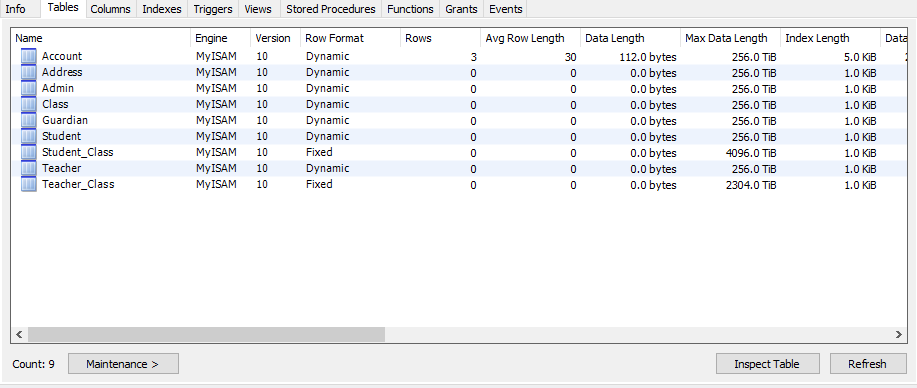
\includegraphics[width=0.5\textwidth]{database_tables}
\end{figure}

\subsection{GUI Work}

\subsubsection{GUI Path and Theme}

The path for the gui was part of the backlog so we could figure out the minimum number of pages we would need to do the things required by this project. This does not mean we are looking to create only the minimum but just get a general idea of how many pages we would need. Also it allowed us to see how the pages were connected and how we expect navigation through the system to work. The rough drawing of the path can be found in the Github repo's sprint two folder.

The other thing we need was to talk to the client about what he wanted for a navigation theme. We came up with three options, first was a button layout on the top and side of the page, second was  drop down menu similar to the way was mac and windows handle navigation in their products. Last was an expanding folder structure similar to that of the content management system Ektron. After consulting with Dr. McGough, he  decided that the more familiar drop down menu would be the easiest and most user friendly option and the option he would prefer we do. This decision allows us to use the built in menu bar functionality of pyqt and should reduce work load on navigation for this project.

Another part of theme is color and design, the color scheme will most likely resemble the academy's color plate, but the improve design will be worked on later. As of now the primary focus is making sure all the functionality works.


\subsubsection{GUI Pages}

The GUI pages for this sprint were the log in page and the landing pages for admin and teachers. The student part of the gui will be php which will be worked on in a future sprint once the functionality is done. Since the student functions are similar to some of the admin or teacher functions most work should port over fairly quickly.

The first page we made was a login in page that takes a username and a password and first checks to see if they exist and are correct within the system. If they are not a dialog saying whats wrong appears and prompts the user again. If the information passes the check the system reads the users permission level and sends them to the corresponding landing page.

\begin{figure}
\caption{Current iteration of the log in page}
\centering
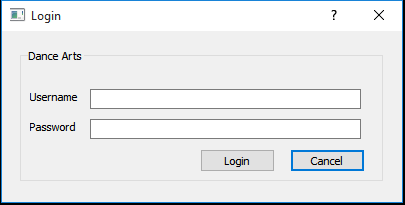
\includegraphics[width=0.5\textwidth]{login_page}
\end{figure}

The other set of pages we need to make to begin writing functionality was the landing pages for the admin and teacher permission levels. These pages show the types of things each can do and allow navigation to the various different functionality that permission level can do. For example the admin landing page has a button to take you to a student options page, from there you select which option you want and will be taken to the page to execute that function. The idea is to start at the landing page and be able to navigate to a specific function in three or four clicks max. The menu bar will also execute navigation and should allow the user to jump to a desired function.\\

\begin{figure}
\caption{Current iteration of the Admin Landing page}
\centering
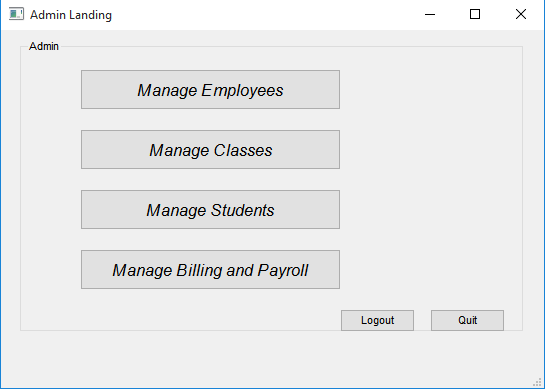
\includegraphics[width=0.5\textwidth]{admin_landing}
\end{figure}

Pages currently being worked on include:

\begin{enumerate}
\item Search pages
\item Modify data page
\item Add information and new information pages
\end{enumerate}


\subsection{Sprint 2 Issues}
Some issues that were encountered during this sprint were:

\begin{enumerate}
\item Running out of time - the group found it hard to complete this sprint on time due to many time draining issues, such as other class work,family matters, midterm exams and a client presentation during this sprint. Mitigation for this issue will be better time management for the team.
\item Inexperience with PyQt - The team ran into some issues that drained on time when working with PyQt, such as looking up information on how to perform a needed task. Mitigation for this issue is mostly experience based as we learn the system and learn how to more efficiently navigate the community the time sink should go down.
\item Team communication - The team found some issues in communicating with one another because of the language barriers within the team. Which in some cases slowed sprint progress. Mitigation for this issue will come with time as the group begin to understand each other better and find efficient patterns of communication.
\end{enumerate}

\subsection{Client Interactions}

Client interactions came in the form of weekly meeting every wednesday at 2:00 p.m. Topics included:

\begin{enumerate}
\item Progress reports on where we are in the project
\item Asking questions to refine functionality and understand academy needs
\item Discuss the future of the project and idea on how to execute them
\end{enumerate}


\subsection{Group Meeting}

The group has a standard meeting time of 4:00-5:00 or 4:00-6:00 MWF and a second meeting time of TTH 10:00 - 12:00

Meeting can continue pass these times if needed, and other times during the weekend. However weekend times fluctuate and do not remain constant from week to week. 

\subsection{Work Distribution}

Marcus:
\begin{enumerate}
\item Gui Path Charts
\item Landing page Construction\\
\end{enumerate}

Dicheng:
\begin{enumerate}
\item GUI Theme Ideas
\item Log In Page and Permission Navigation\\
\end{enumerate}


Together:
\begin{enumerate}
\item Wrote and talked through database and construction
\item Got database running
\item GUI page breakdown based on user stories and product backlog
\item Coded some functionality
\end{enumerate}


\section{Sprint Report \#3}

Sprint Report \#3


\subsection{Team Members:}
Marcus Berger
\\Dicheng Wu\\
\textbf{Sponsor:}
\\Jeff McGough
\\

\subsection{Prototype Progress}
The progress is being made on the simpler functions of the projects including search, updates, and role sheets. As of now the prototype is in a state of some working functionality on the admin and teacher side. The pages are not yet tied together but the complete functions function independently. Several GUI pages are complete or in a working state to compliment these functions. The back end database has been slightly updated to adjust to the needs of the project. Lastly the prototype has reached a state where testing can be conducted on parts of the project, more information is given later in this document.

\subsection{Project deliverables of Sprint 3:}

\begin{enumerate}
\item Student search page 
\item Employee search page
\item Add a class to the database
\item Update teacher and student information pages
\item Modify clothing requirements for a class
\item Generate a class role sheet
\item Assign teacher to a class
\item Ability to add and subtract students from a class  
\end{enumerate}


\subsubsection{Sprint 3 Backlog:}

\begin{enumerate}
\item Queries in database to retrieve student and employee information
\item Query and insert information needed to create and new class and produce a results page.
\item Query database to produce class role sheet
\item Create clothing requirement update function, and add clothing function for teachers and admin
\item Create update query to assign teachers to a class
\item Create ability for employee to look up and modify student registration info
\item Add and subtract students from a class
\item Sprint 3 Review
\item Create Client presentation
\item Documentation for semester
\end{enumerate}

\subsection{Search Pages}
The first page tackled this sprint was the search page. The page takes user input and searches based on name using a fuzzy search. Also included in both searches is an advanced search option that allows the user to check boxes corresponding to the fields in the database, which allows the user to search in more versatile ways. Lastly the user can click on a student to pull up all of their information and modify it as needed.


\begin{figure}
\caption{Search Pages}
\centering
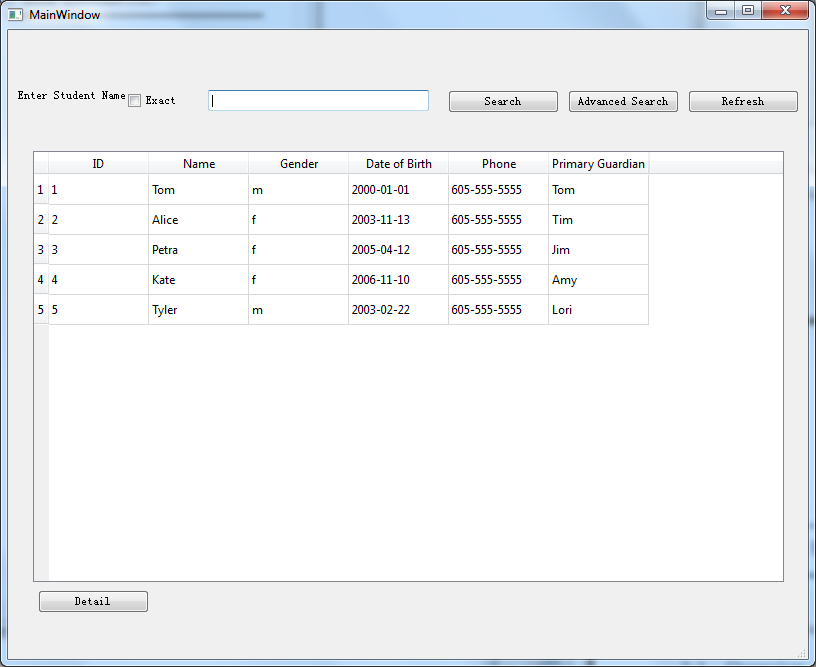
\includegraphics[width=0.5\textwidth]{search.png}
\end{figure}

\subsection{Add A Class}
Clicking on the "Add a Class" button on the admin landing page will open a dialog. From this dialog box the user can type in information to a add a class. These fields include class name, cost, start and end times, day, clothing requirements, class description, start and end dates, and the age range for the class.  At the time of class creation only name, is a required field. When the submit button is clicked a message box will pop up to confirm the database submission before submitting to the database  

\subsection{Role Sheet}
This page generates a list of classes teachers are currently teaching. Teacher can see who is taking his/her class by selecting the corresponding class on the list and can print this list as a pdf. 

\subsection{Update Pages}
These pages are fairly simple to explain sometimes the user will need to add or alter a record of some kind these pages need to be able to do that in a simple and concise way. The update pages worked on in this sprint include student information from the employee side, updating teacher information and updates to clothing requirements for a class. Most of these page will just produce a form where information can be displayed and updated.

\subsection{Assign Teacher to a Class}
This page allows an admin to select a class, clicking on a class pulls up a list of available teachers to select to teach the class. Clicking on a teacher will pull up a message box to confirm the selections before submitting to the database. The available teachers are selected based on the start time of the selected class and the end time of the classes already being taught by each teacher. If the class times overlap then that teacher will not show up in the available teachers list.

\subsection{Sprint 3 Issues}
Some issues that were encountered during this sprint were:

\begin{enumerate}
\item Time - While not as much of a problem as it was in sprint two the group still found itself running low on time. The lead gained during Christmas break should reduce the issue in phase 2.
\item Inexperience with pyqt - While still a small issue the experience of the team is growing and while some issues still exist such as needing to look up information at times, the issues are lessened from the last sprint.
\item Team communication - The team found some issues in communicating with one another because of other projects and assignments. Which in some cases slowed sprint progress. Mitigation for this issue will be to more strongly impose a schedule in phase 2.
\end{enumerate}

\subsection{Client Interactions}

Client interactions came in the form of weekly meeting every Wednesday at 2:00 p.m. Topics included:

\begin{enumerate}
\item Progress reports on where we are in the project
\item Asking questions to refine functionality and understand academy needs
\item Discuss the future of the project and idea on how to execute them
\end{enumerate}


\subsection{Group Meeting}

The group has a standard meeting time of TTH 10:00 - 12:00 and once during the weekend usually from 1:00-5:00 

Meeting can continue pass these times if needed, and other times during the weekend. However extra weekend times fluctuate and do not remain constant from week to week. 

\subsection{Work Distribution}

Marcus:
\begin{enumerate}
\item Add a class
\item Assign teacher to class
\item Update teacher page
\item Update clothing
\item documentation
\item trello management\\
\end{enumerate}

Dicheng:
\begin{enumerate}
\item Search Pages
\item Role sheet
\item Modify student information
\item Add and Subtract students from a class
\item Navigation to teacher or admin page\\
\end{enumerate}


Together:
\begin{enumerate}
\item Updated database construction
\item GUI page breakdown based on user stories and product backlog
\item Coded some functionality
\end{enumerate}

\section{Sprint Report \#4}

Sprint Report \#4


\subsection{Team Members:}
Marcus Berger
\\Dicheng Wu\\
\textbf{Sponsor:}
\\Jeff McGough
\\

\subsection{Prototype Progress}
During sprint 3.5 the team organized the functionality and tied them together to create the working prototype. Other updates were made to fix known bugs and add a class search. While the team worked on putting the project together smaller bugs or needed pages that were implied by user stories were tackled as they came up. This resulted in to much time being used, so the student interface was not tackled. The student interface has since been dropped from the clients project requirements due to time.

Sprint 4 was dedicated to payroll and billing. First the client rewrote the user stories to provide more clarity to the team. After this the user stories were tackled by the group to produce the first draft of the payroll and billing interface. This included logging hours, payments, fees, rates, credits, and discounts. After this was done the team demoed the project for the client and got notes on the project as a whole. These notes will be tackled as part of the backlog in the next sprint.


\subsection{Project deliverables of Sprint 3.5 and 4:}
Sprint 3.5 had no defined deliverables, and was mostly clean up.

Sprint 4 deliverable was the first draft of the payroll and billing interfaces and functions, layed out in the user stories below.



\subsubsection{Sprint 3.5 Backlog}

\begin{enumerate}
\item Fix Assign Teacher to Class Dialog Bug
\item Add Class Search
\item Complete Role Sheet
\item Tie Functions Together
\item Fix Smaller Bugs
\end{enumerate}

\subsubsection{Sprint 4 Backlog:}

\begin{enumerate}
\item View Teaching History
\item Look at The Current Amount Someone Owes
\item Generate an Invoice For The Amount Due
\item Look at Billing History
\item Apply Credits to a Students Account
\item Enter the Tuition and Fees Rate
\item Give Early Registration Discounts
\item Enter Staff Pay Rates
\item Enter a Full Payment for One Student 
\item Enter a Full Payment for Several Students
\item Enter Payments From Multiple Sources For One or More Students
\item Compute Teacher Wages 
\item Enter Staff Hours
\item Give Prorated Refunds 
\end{enumerate}

\subsection{Sprint 3.5}
During sprint 3.5 Class Search was added this page follows the same format as other search pages created in previous sprints. Also completed fixes to the assign teacher to class bug, role sheet completeness, and a few other minors bugs. At the end of the sprint the team tied what we had together so the product could run as a unit starting from the log in screen.

\subsection{Prorated Refunds}
The prorated refunds code will keep track of how much a class costed a student. If the student drops a class it will refund the remaining worth of the class to the students school credit field. This file is still in progress.

\subsection{Enter Staff Hours}
This page needs to undergo changes after meeting with client. The new version will allow a teacher to log their in class hours, office hours, trip hours, etc. These hours will then be paid out at their different rates respectfully. The hours will be logged as single numbers not by days or weeks.

\subsection{Enter Teacher Wages}
This was handled in the database in previous sprints assuming one pay rate. However in talks with the client the academy pays different pay rates based on what part of academy work they are doing. So the page will need to be updated once the list of possible pay rates have been provided by the client.

\subsection{Enter Tuition Rates and Fees}
These pages allow the user to look at the current tuition rates and fees. The user can then update existing rates, add new rates, or remove rates that are no longer needed. Tuition rates are logged in the database as flat minute rates. The user can enter new rates in the form of minutes or hours.

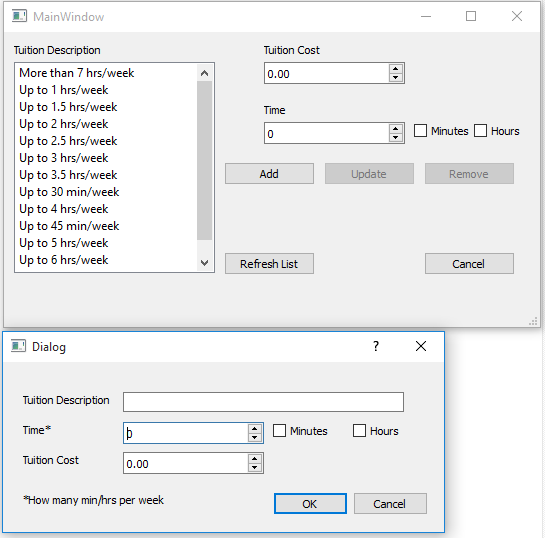
\includegraphics[scale=0.5]{tuitionRates.png}

\subsection{Teacher History}
This page includes several components. Firstly, user can use this page to find a specific teacher by entering a full or partial name of teachers. Secondly, users can click the history button to open up another window which has a list of classes the teacher has taught.\\

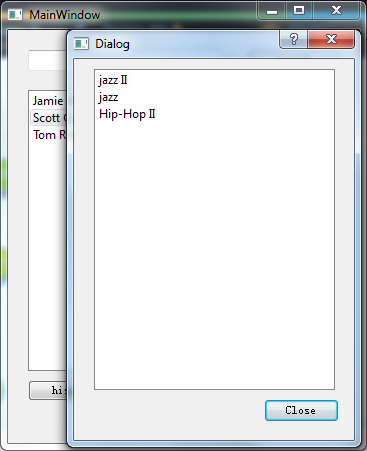
\includegraphics[scale=0.5]{teacherHistory.png}

\subsection{Set Semester}
This page helps users to set the current semester from pool of semester and add a new semester to the system.

\subsection{partial payment}
This page includes several components. Firstly, user can use this page to find a specific student by entering a full or partial name of students. Secondly, users can click the pay button to open up another window which asks user to input amount of money paid, payment's method and semester paid. The user also can choose single or multiple students at one time. \\
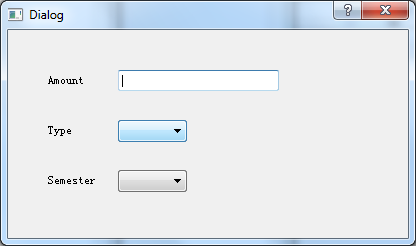
\includegraphics[scale=0.5]{payment.png}

\subsection{Student's owe}
This page includes several components. Firstly, user can use this page to find a specific student by entering a full or partial name of students. Secondly, users can click the statement button to open up another window which shows the amount of students paid, the amount of students due and the balance of student's account. Users also can print the invoice generated by the window.\\
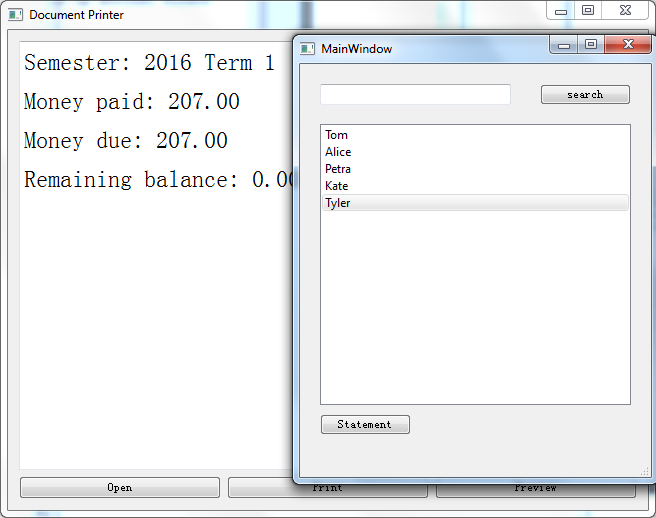
\includegraphics[scale=0.5]{invoice.png}

\subsection{enter payment}
This page includes several components. Firstly, user can use this page to find a specific student by entering a full or partial name of students. Secondly, users can click the clear button to clear the due of selected students. Users can select single or multiple students at one time.\\
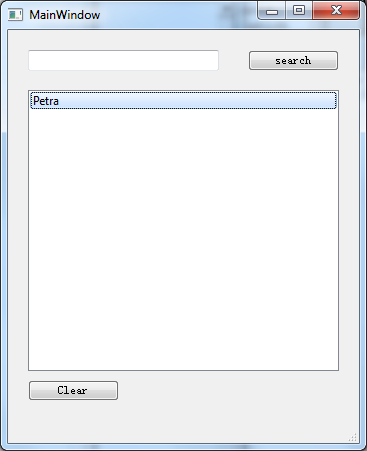
\includegraphics[scale=0.5]{enterPayment.png}

\subsection{bill history}
This page includes several components. Firstly, user can use this page to find a specific student by entering a full or partial name of students. Secondly, users can click the statement button in order to get the list of payments. In addition, user can print the bill history.\\

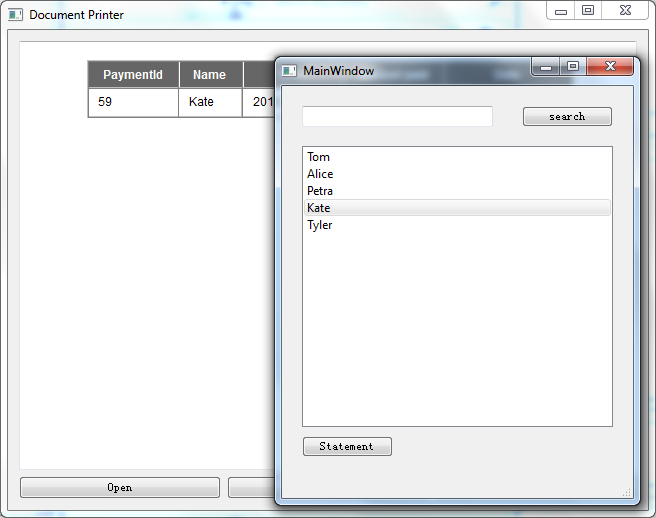
\includegraphics[scale=0.5]{billHistory.png}

\subsection{Sprint 3.5 and 4 Issues}
Some issues that were encountered during this sprint were:

\begin{enumerate}
\item During winter break the team wanted to tackle the student interface app. Building other required pages in the main local GUI made this a problem. Therefore while some implied GUI pages where fixed and created, the team was unable to get to the student interface. As a result the student interface was removed from the project requirements.
\item Spring semester ramp up - Coming back from a month break meant that the team needed to ramp back up and get used to the new classes and new commitments. This cause the team to move slower then it should have in this sprint. 
\item Team communication - The meeting this sprint were less effective as teams members would have other commitments, or in some cases lack the drive to do the work. This lessen as the sprint continued, but sometimes still came up.
\item Requirement Confusion - At times during this sprint the requirement were confusing. This resulted in a rewrite of the requires for payroll and billing to provide more clairity and adjust for dropping the student interface. The rework helped the team greatly, however the user stories still sometimes left out core part of how the academy does its work compared to other places. This resulted in spending more then the usually time speaking with the client, and group friction.
\end{enumerate}

\subsection{Client Interactions}

Client interactions came in the form of requires reviews and a demo of the prototype at the end of the sprint. Topics included:

\begin{enumerate}
\item Progress reports on where we are in the project
\item Asking questions to refine functionality, understand academy needs, and update requirements.
\item Discuss the future of the project and idea on how to execute them.
\item Prototype the current version of the prototype.
\end{enumerate}


\subsection{Group Meeting}

The group has a standard meeting time of TTH 10:00 - 12:00 and once during the weekend and at home as needed.  

Meeting can continue pass these times if needed, and other times during the weekend. However extra weekend times fluctuate and do not remain constant from week to week. 

\subsection{Work Distribution}

Marcus:
\begin{enumerate}
\item 3.5 Fix Assign Teacher Bug
\item 3.5 Update GUI Functions, Minor Additions and Fixes
\item 3.5 Tie Various Functions Into a Single Prototype
\item Prorated Refund (Still in Progress)
\item Enter Teacher Hours (Still in Progress)
\item Teacher Pay Rates (Needs Updated With New Information)
\item Early Registration Discounts
\item Gives Credits
\item Enter and Update Tuition Rates
\item Enter and Update Fee Rates and Type (Needs Updated With New Information)
\item documentation
\item trello management\\
\end{enumerate}

Dicheng:
\begin{enumerate}
\item 3.5 Tie function together
\item 3.5 Class Search Pages
\item 3.5 Updated Role sheet
\item 3.5 Research Linux Boxes
\item 3.5 Tie Functions Together Into a Single Prototype
\item Enter Payments From Multiple Sources For One or More Students
\item Look at The Billing History
\item Enter a Full Payment For One or More Students
\item Enter Payments From Multiple Sources For One or More Students
\item Generate an invoice for the amount due (Needs Updated)
\item Look at a The Current Amount a Student/Family Owes
\item View Teaching History
\item Auto and Manual discount giving
\item Set semester
\end{enumerate}


Together:
\begin{enumerate}
\item Updated database construction
\item GUI page breakdown based on user stories and product backlog
\item Coded some functionality
\end{enumerate}

\section{Sprint Report \#5}

Sprint Report \#5


\subsection{Team Members:}
Marcus Berger
\\Dicheng Wu\\
\textbf{Sponsor:}
\\Jeff McGough
\\

\subsection{Prototype Progress}


Sprint five was dedicated to finishing the last of the functions and clean up of the project. First the client modified  some requirements for the team. After this the user stories remaining from sprint four were tackled by the group to produce the remaining payroll and billing interface. This included logging hours, and payments. After this was done the team started on bug fixes and quality of life updates such as new buttons and removal functions. The team is currently working on finishing up the student registration, and tax calculation for wages. If progress continues at this rate the prototype should be completed functionally however without some work the prototype may not reach some of the teams desired standard.


\subsection{Project deliverables of Sprint 5:}

Sprint 5 deliverables were the remaining functionality for the project. If the sprint was successful the main project will be done or very close to done functionally at the end of the sprint.


\subsubsection{Sprint 5 Backlog}

\begin{enumerate}
\item Admin and teacher update crossover
\item Ignoring case in address forms
\item Add rejected students to approved/ reject and provide current status
\item Multiple pay rates
\item Admin list function
\item Enter staff hours
\item Sprint 4 rollover (remaining payroll functions)
\item Add and remove class location
\item Removal Functions (Admin, Class, Student, Teacher)
\item Refunds and check boxes for fees and tuition
\item Quality of life updates to some functions
\item Bug Fixes
\item Student registration
\item Employee wages
\item Begin User Guide for documentation
\end{enumerate}


\subsection{Sprint 5}
During sprint five the team tackled the remaining functionally, bugs, and quality updates in an attempt to finish the base project. Removal functions to clean out the database were added, and some client requested quality of life updates were added. Bugs and glitches were patch up in many functions. Another job of this sprint was to finish the rollover from sprint four since some payroll functions still needed work. Lastly the team tackled student registration since the student interface was dropped from the project requirements in sprint 4. The registration is still in progress at this time, as the team failed to complete this functionality in time for the end of the sprint.

\subsection{Prorated Refunds}
The prorated refunds code will keep track of how much a class costed a student. If the student drops a class it will refund the remaining worth of the class to the students school credit field. This file has now been completed.

\subsection{Enter Staff Hours}
This page needed to undergo changes after meeting with client. The new version will allow a teacher to log their in class hours, office hours, trip hours, etc. These hours will then be paid out at their different rates respectfully. The hours will be logged as single numbers not by days or weeks. This function is now completed

\subsection{Enter Teacher Wages}
This was handled in the database in previous sprints assuming one pay rate. However in talks with the client the academy pays different pay rates based on what part of academy work they are doing. So the page will need to be updated once the list of possible pay rates have been provided by the client. This pages and its updates are still in progress. \\

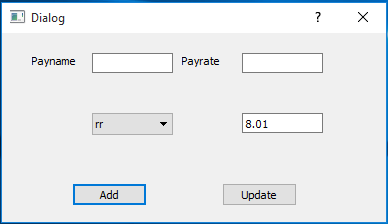
\includegraphics[scale=0.5]{payRates.png}

\subsection{Enter Tuition Rates and Fees}
Updated these pages to provide quality of life updates to the function requested by the client.\\

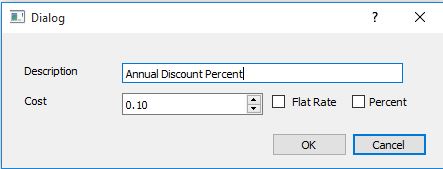
\includegraphics[scale=0.5]{feeDialog.png}

\subsection{Bug Fixes}
During the course of testing and the client meeting some bugs or inconsistencies were discovered within the project. The bugs found and fixed are:

\begin{enumerate}
\item Student search was not showing all the students. Status: Fixed
\item Search edit need to be turned off and advance search modifications. Status: Fixed
\item Search, role, and schedules need to have dynamic not static times. Status: Fixed
\item Allow for time changes on schedule. Status: Fixed
\item Some of the back buttons in the teacher interface did not work correctly. Status: Fixed
\item Forms seem to be bugged at times, however can not recreate bug. Status: In testing possibly fixed.  
\end{enumerate}

\subsection{Updates Crossover}
One of the updates that needed to be completed this sprint was the need for admin and teacher updates to crossover if something was changed. This means that if someone is an admin and they update there phone number through the "update my information form" then the phone number will be updated in both the teacher table and the admin table. This way the system will not have conflicting information in different places. 

\subsection{Approved/Rejected Student Updates}
A update requested by the client was the ability to see rejected students in the approved/rejected pages just in case the academy changed its mind about a student. The page underwent slight modifications to the way information was displayed to make this change efficiently\\

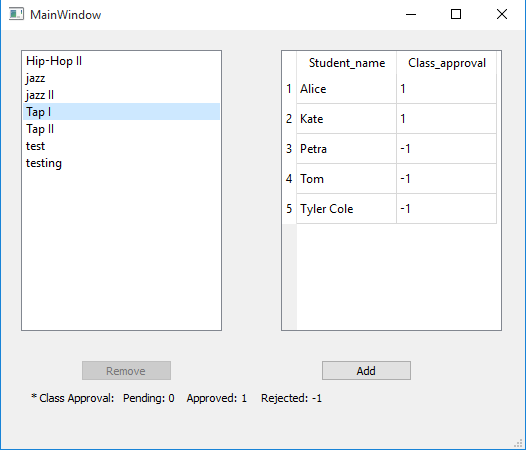
\includegraphics[scale=0.5]{newAddStudent.png}

\subsection{Admin List}
In creating some of the updates it became clear that a specific admin list was needed to see who had admin access to the system. This was done through a simple list view of the names that can then be selected to display more detailed information.\\


\subsection{Add/Remove Locations}
Another requested feature was the ability to add and remove locations for classes in the database. This feature is necessary because the academy sometimes teaches classes in different places based on need. The team accomplished this using a simple dialog that connects to the location table in the database. When the user updates or adds a new class the location combo box provides a list of locations in the database and an add location option.\\

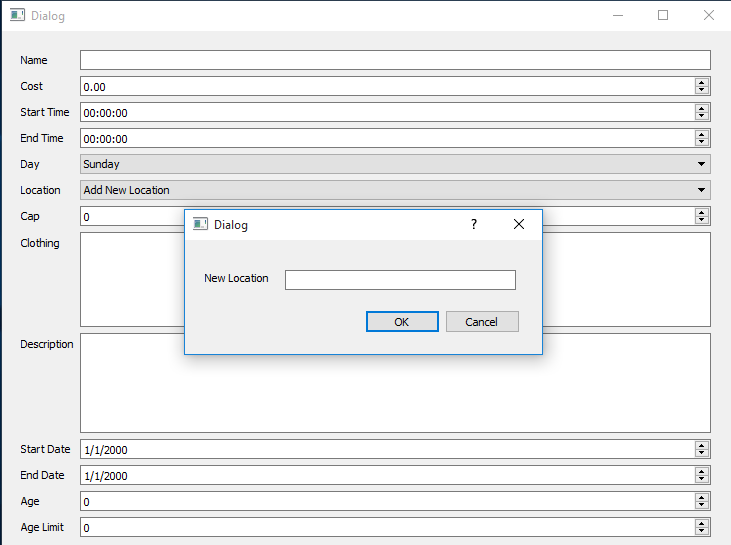
\includegraphics[scale=0.5]{newLocation.png}


\subsection{Removal Functions}
These are simple functions that pull up a dialog box where the user can select a name and remove all the information related to that user from the system. The removal functions that exist in the system are: teacher, admin, student, and class. Teacher will remove that persons information from the system. Admin removes that persons admin rights and then ask if the whole user should be removed.\\

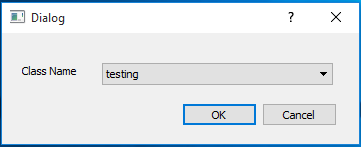
\includegraphics[scale=0.5]{removal.png}

\subsection{Sprint 5 Issues}
Some issues that were encountered during this sprint were:

\begin{enumerate}
\item Spring semester ramp up - This was by far the biggest issue this sprint and the main cause of the failures this sprint. Other classes  up to the point of blocking work on many projects. Staggered due dates meant that when the team wanted to work, there was always another projects that needed to be completed in a short amount of time. By the end much of our time had been taken and the sprint began to fall behind.  
\item Requirement redefining - Due to drop the student interface the functionally needs to be added to the GUI which created some extra work for the team. 
\item Failure to complete backlog - The team did not finish all of the assign backlog this sprint.
\end{enumerate}

\subsection{Client Interactions}

Client interactions came in the form of required reviews and a demo of the prototype at the end of the sprint. Topics included:

\begin{enumerate}
\item Progress reports on where we are in the project
\item Asking questions to refine functionality, understand academy needs, and update requirements.
\item Discuss the future of the project and idea on how to execute them.
\item Prototype the current version of the prototype.
\end{enumerate}


\subsection{Group Meeting}

The group has a standard meeting time of TTH 10:00 - 12:00 and once during the weekend and at home as needed.  

Meeting can continue pass these times if needed, and other times during the weekend. However extra weekend times fluctuate and do not remain constant from week to week. 

\subsection{Work Distribution}

Marcus:
\begin{enumerate}
\item Bug fixes
\item Removal functions
\item Admin and teacher update crossover
\item Ignore Case on address forms
\item Add rejected students to appoved/ reject and provide current status
\item Add/remove class location
\item Prorated refunds
\item Quality of life updates
\item Sprint report
\item Start User Guide
\item Trello management\\
\end{enumerate}

Dicheng:
\begin{enumerate}
\item Bug fixes
\item Pay rates
\item Admin list
\item Staff hours
\item Student registration (in progress)
\item Wage calculations (in progress)
\end{enumerate}


Together:
\begin{enumerate}
\item Updated database construction
\item Update prototype structure
\item Coded some functionality
\end{enumerate}

